\section{Arquitetura}
    O sistema foi construído utilizando a arquitetura cliente-servidor, em que o back-end (que contempla a lógica do negócio e o gerenciamento de dados, arquivos etc) fornecerá uma \ac{api} a ser consumida pelo cliente \gls{JavaScript}, em execução no navegador do usuário. Fez-se uso dos recursos oferecidos pela \ac{aws}, a fim implantá-lo.

    Para prover arquivos estáticos, o que inclui a própria aplicação \ac{JavaScript}, folhas de estilo \ac{css}, arquivos carregados por usuários, entre outros, o serviço de armazenamento \ac{s3}, com a mediação do CDN CloudFront, foi aplicado.

    O back-end é executado em instâncias de máquinas virtuais do \ac{ec2}, o que possibilita a configuração de escalonamento automático e balanceamento de carga, garantindo escalabilidade à \ac{api}. Por fim, um banco de dados relacional é criado através do serviço de banco de dados relacional. O diagrama da \autoref{arquitetura-sistema} demonstra a arquitetura descrita.

\begin{figure}[H]
    \centering
    \caption{\label{arquitetura-sistema}Arquitetura do Sistema}
    \frame{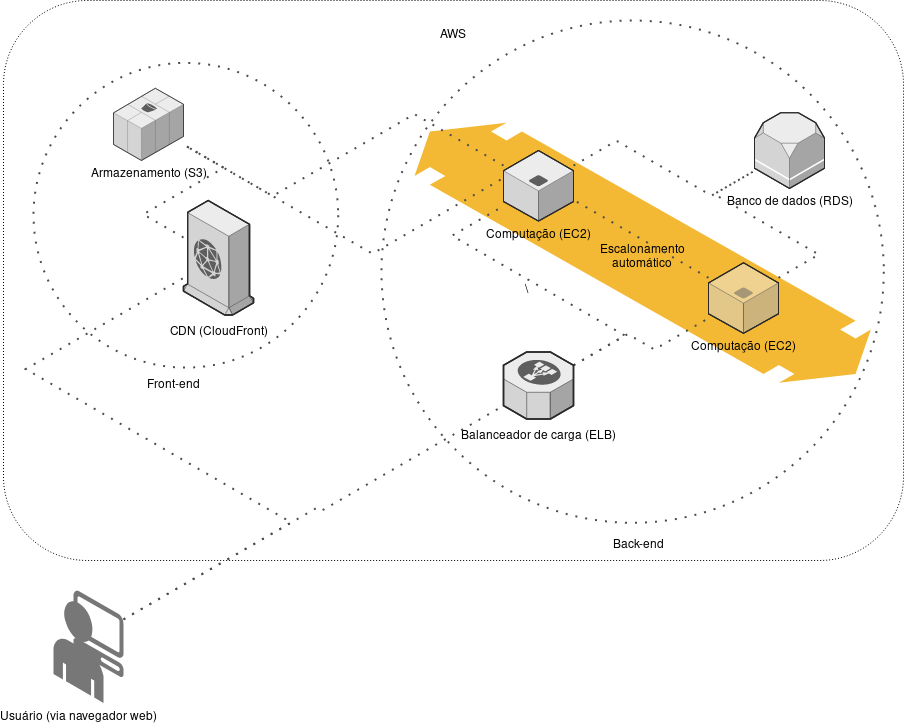
\includegraphics[width=0.8\textwidth]{anexos/arq_fig.png}}
    \fonte{Os autores}
\end{figure}

\subsection{Análise de Requisitos}
    A etapa de análise de requisitos é a parte que os \ac{dt} elaboram as funcionalidades e regras do sistema. Também é definido junto com \ac{po} os requisitos a fim de elaborar as histórias para que esses itens entrem como candidatos para a \gls{sprint-planning}. Portanto, os itens são votados na planning para que os \ac{dt} iniciem o desenvolvimento na sprint.
    
\subsubsection{Regras de Negócio}
Foram determinadas dez regras para a nossa plataforma. O \autoref{regra-negocio} contém as \gls{regras-negocio} com seu determinado identificador e a descrição da regra.
\begin{quadro}[H]
	\centering\footnotesize
	\caption{Regras de Negócio}
	\resizebox {.72 \textwidth }{!}{
        \label{regra-negocio}
        \begin{tabular}{|l|p{8cm}|}
        \hline
        \thead{Identificador} & \thead{Descrição} \\ \hline
        RN01 & Os usuários menores de 18 anos não podem realizar o cadastro na plataforma.           
        \\ \hline
        RN02 & Uma vaga publicada pode ficar disponível por até 90 dias, após esse período deve ter opção de renovação ou inativação automática.
        \\ \hline
        RN03 & A exibição de visitas na vaga é exibida em área logada e somente para o perfil família ou agência.
        \\ \hline
        RN04 &  Perfil au pair, família e agência podem ser avaliados por comentários e ter a opção de conceder nota, mas não podem se autoavaliar.
        \\ \hline
        RN05 & Somente au pair podem receber o consolidado das vagas publicadas nos últimos 7 dias por e-mail.
        \\ \hline
        RN06 & Um au pair pode se candidatar em uma ou mais vagas.
        \\ \hline
        RN07 & Família ou agência podem publicar vagas de forma ilimitada.
        \\ \hline
        RN08 & Para cada vaga publicada será cobrado um valor especificado na tabela vigente de preços, considerando se será dado destaque ou não na exibição.
        \\ \hline
        RN09 & Uma família e/ou uma agência podem ter acesso ao publicador.
        \\ \hline
        RN10 & Agência ou família não podem ter acesso aos dados de contatos uma da outra.
        \\ \hline
        \end{tabular}
    }    
\fonte{Autores}
\end{quadro}